\cite{tramèr2020ensemble} addressed the issue of black-box attacks. They found that the testing
regime used previously did not adequately assess whether adversarially trained models can handle
black-box adversarial examples in general. Specifically, they found that the linear black-box
attacks used (for example, FGSM\cite{goodfellow2015explaining}) were not good at reaching the
maximum in the min-max problem discussed in \cite{madry2019deep}, and that white box attacks turn
out to be not as good as black-box attacks on models that have been trained with first-order, single
step attacks. Further, it is possible that white-box attacks on these adversarially trained models
transfer poorly when used as part of a black-box attack on \textit{non-adversarial} models.

They came to these conclusions first by probing the loss function space with respect to a
two-dimensional subspace whose axes are essentially the sign of the gradient and a vector
perpendicular to it (likely inspired by \cite{goodfellow2015explaining}) scaled by increasing
adversarial perturbation magnitudes. At each point, two noise vectors generated from the first and
second magnitudes multiplied by the sign of the gradient and its orthogonal counterpart,
respectively, were added to the non-adversarial example (we will call these scaled vectors $a$ and
$b$, again, respectively). This generated a three-dimensional map, with the $z$ axis representing
the loss at the adversarial example represented by the point generated from the addition of $a$,
$b$, and the original image (axes represented the $L_{\infty}$ magnitude of $a$ and $b$). See figure
\ref{badgradients} for an example of a plot. They point out that the gradient at small perturbation values
points in a drastically different direction compared to the direction that would lead to the largest
increase in loss. They state that this explains both why white-box attacks on the aforementioned
adversarially-trained models do not work well on both the adversarially-trained and
non-adversarially trained models: this gradient does not represent the most effective direction for
ascent. Therefore, testing in the signed direction gives a false sense of security w.r.t. the
defended model, and these new images also, as a result, do not perform well as a black-box attack
against undefended ones. They call this phenomenon \textit{gradient masking}.
\begin{figure}[th]
    \begin{center}
        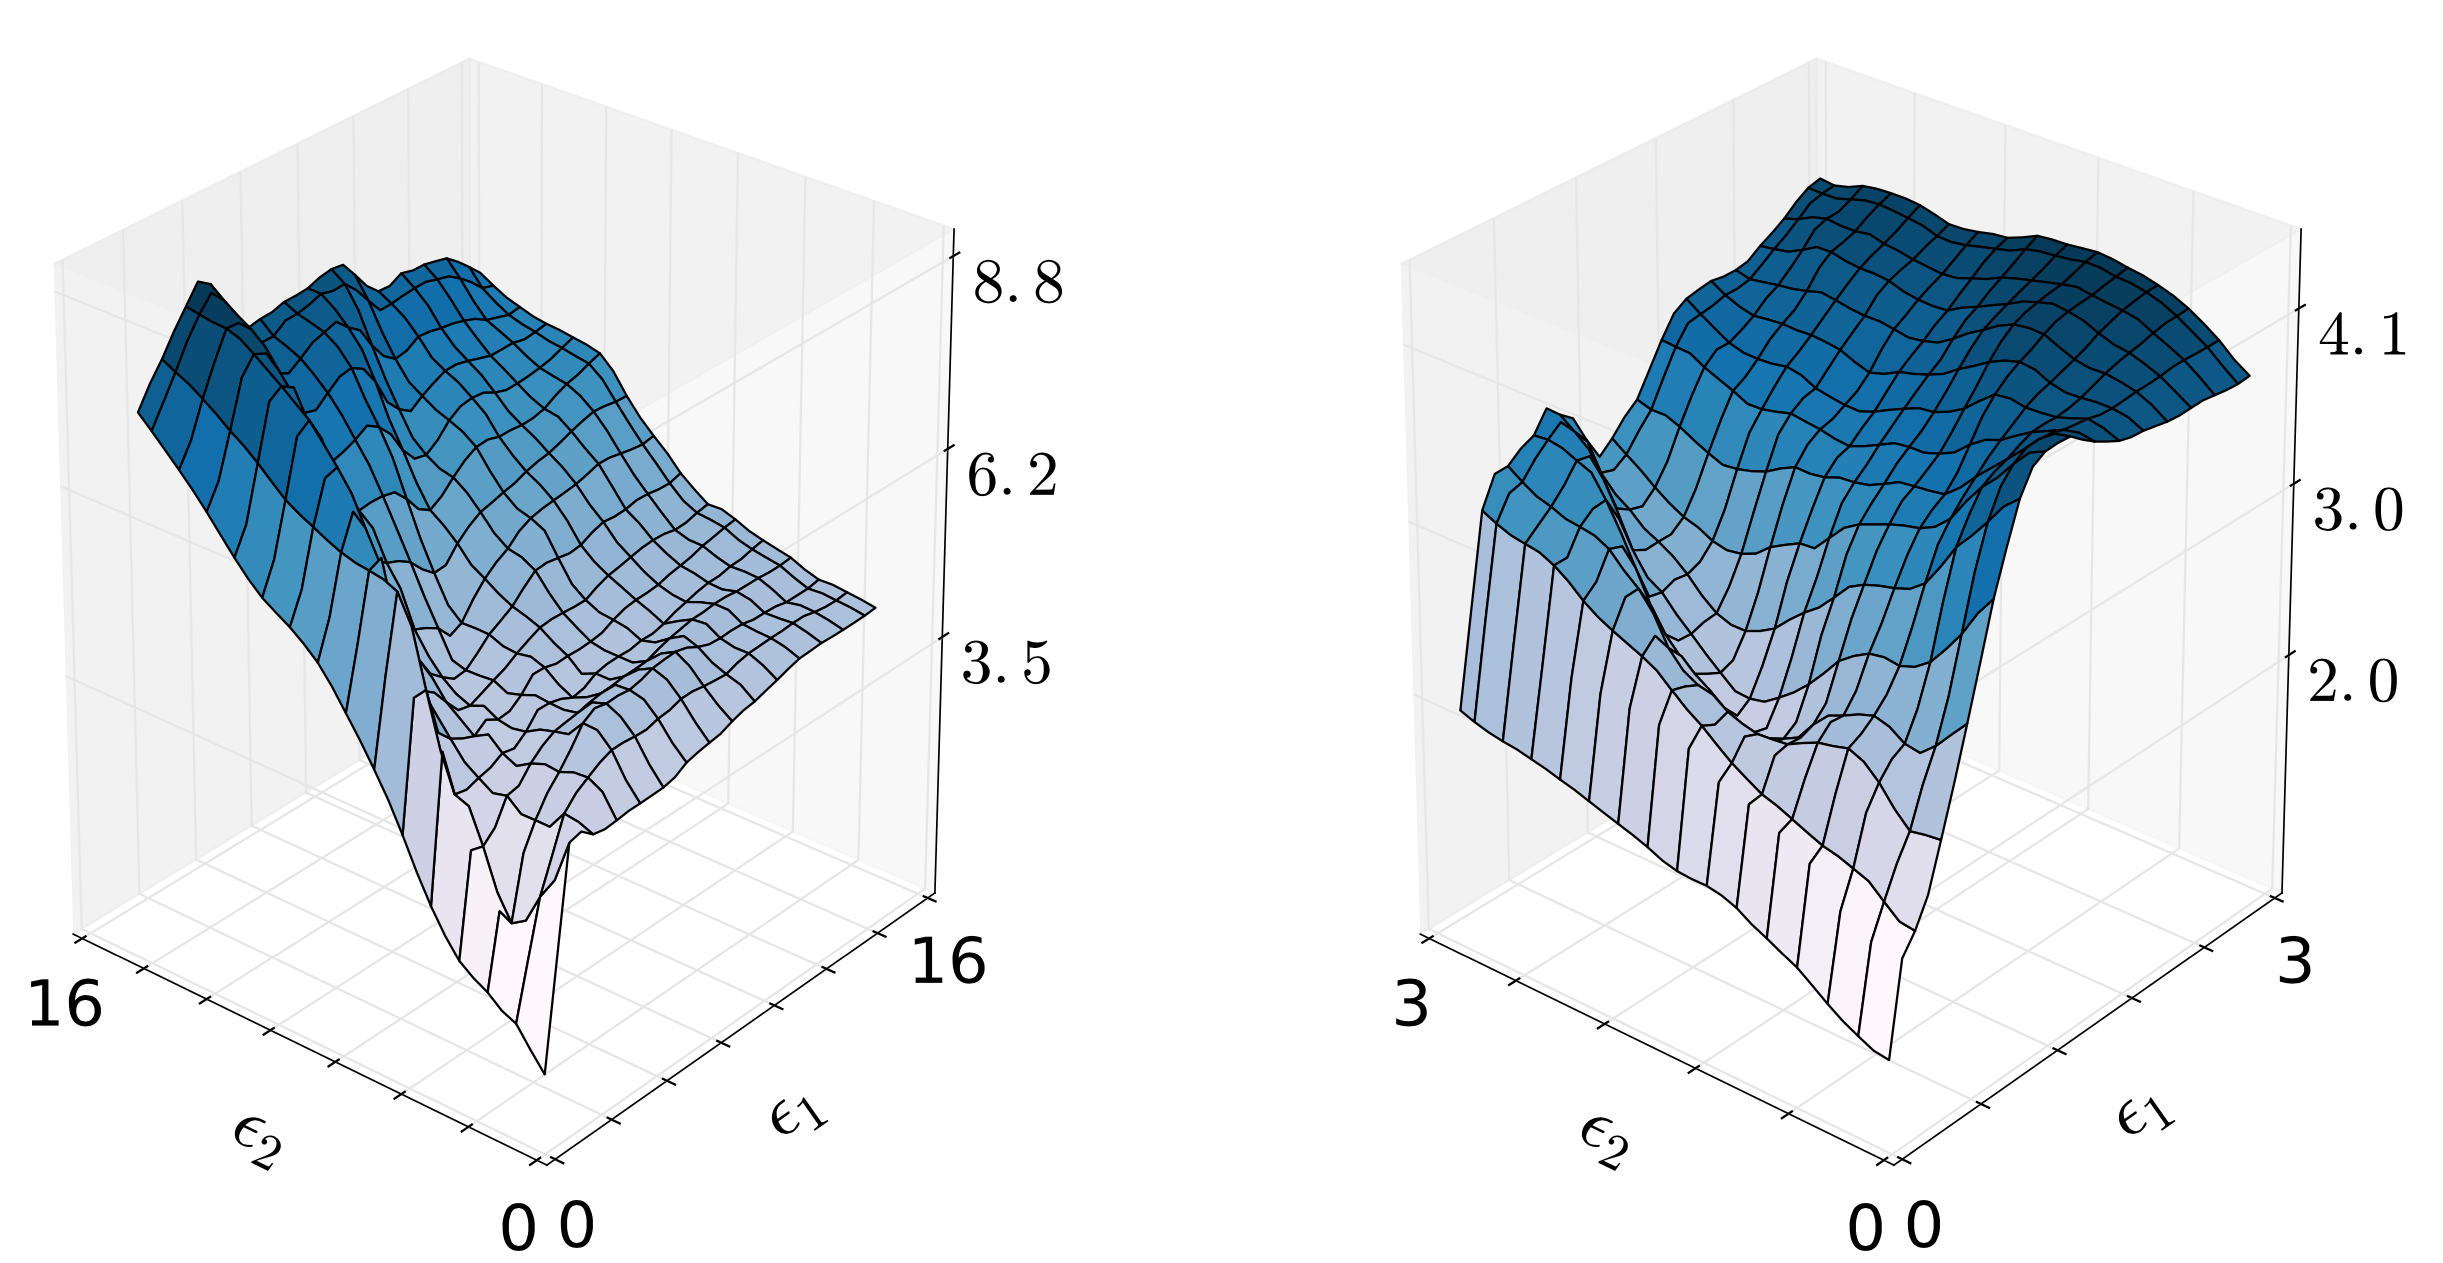
\includegraphics[width = \linewidth]{Friendly/LaTeX/figures/maskinggraphs.png}
        \caption{An example of gradient masking. The gradients in the data point's immediate
                 vicinity point one direction, while the actual maximizer is in the other direction.
                 Image is a snapshot from \cite{tramèr2020ensemble}[figure 4].}
        \label{badgradients}
    \end{center}
\end{figure}

To tackle this issue, they introduced \textit{Ensemble Adversarial Training}. In this technique,
not only do they train on white-box adversarial examples, but they also incorporate black-box
examples generated from non-adversarially-trained models. Each model contributed the same number
of adversarial examples, but only one model's adversarial examples were used each iteration. It
appears that only adversarial examples were in the training set. They found that this defense had
much better black-box resistance, and it eliminated cases in which the black-box attack was better
than white-box.